\documentclass[12pt, letterpaper]{article}
\usepackage[spanish]{babel}
\usepackage[utf8]{inputenc}
\usepackage{graphicx}
\usepackage{subcaption}
\usepackage[hidelinks]{hyperref}

%Esta propuesta debe contener: 


%- Otros antecedentes de relevancia que aporten a la glorificación del trabajo a desarrollar
%-Esta propuesta debe ser entregada a su patrocinante y éste, en señal de acuerdo y aceptación de la misma, la debe enviar a la jefatura de carrera.


\begin{document}
%portada
\begin{titlepage}
	\begin{figure}
		
		\begin{subfigure}[b]{0.5\textwidth}
			
\includegraphics[scale=0.45]{figures/diicc.png}
		\end{subfigure}
		\hfill
		\begin{subfigure}[b]{0.1\textwidth}
			
\includegraphics[scale=0.4]{figures/escudo_udec.png}
		\end{subfigure}
	\end{figure}
	
	\centering	
	\par\vspace{1cm}
	{\scshape\LARGE Universidad de Concepción \par}
	{\scshape Ingeniería civil informática \par}
	\vspace{1cm}
	{\scshape\Large Propuesta memoria de título\par}
	\vspace{1.5cm}
	{\huge\bfseries Diseño e implementación de sistema de fiscalización de procesos de compostaje\par}
	\vspace{2cm}
	{\Large\itshape Francisco Flores Mellado\par}
	\vfill
	prof. patrocinante\par
	Dr.~Pedro \textsc{Pinacho Davidson}

	\vfill

% Bottom of the page
	{\large \today\par}
\end{titlepage}

\section{Introducción}
%contexto del trabajo
%descripción del problema
%forma general de solución propuesta con resultados esperados
Actualmente el país presenta un creciente desarrollo de la actividad del compostaje como una alternativa a la gestión de residuos orgánicos, los cuales provienen principalmente de restos de alimentos de mercado o ferias libres y de vegetales producto de las podas de parques y jardines. \\
El compost se produce a base de residuos orgánicos y específicamente suele ser utilizado como mejorador de algunas propiedades físicas del suelo como son su estructura, drenaje, aireación, retencion de agua y nutrientes, prevención de la erosión del suelo, recuperación de suelos degradados y superficies alteradas sin uso agrícola. El compostaje se presenta como una alternativa a la quema agrícola.\\
Con el fin de mantener un estándar en la producción, mantenimiento, almacenaje, transporte y posterior venta de compost, es que se creó una norma que busca, en términos generales, promover la gestión adecuada de los recursos sólidos orgánicos generados en el territorio nacional, evitar la producción de plagas, junto con promover y fomentar el desarrollo de la industria nacional de compost. En ese sentido, la norma cubre aspectos relacionados a la clasificación del compost, requisito de materias primas, requisitos del producto compostado, los que incluyen requisitos sanitarios y físico químicos. Estos últimos, abarcan desde contenido de nutrientes, capacidad de rehidratación, pH, materia orgánica, hasta olores y humedad.\\
El ornagismo a cargo de supervisar el cumplimiento de estas normas y la calidad del compost, para su uso de agricultura orgánica, es el Servicio Agrícola y Ganadero (SAG) que depende del ministerio de agricultura. El SAG no tiene la capacidad de fiscalizar todos estos procesos, pero sí otorga los permisos necesarios a organismos de certificación nacionales o extranjeros, públicos o privados, para ingresar al Registro de Entidades Certificadoras de Productos Orgánicos, quienes cumplen las formalidades, requisitos y protocolos técnicos y profesionales necesarios para la ejecución de las labores de certificación. Estos organismos están enfocados principalmente a la actividad industrial de fabricación de productos agrícolas. Por otro lado, también existe el Sistema de auto certificación con fiscalización directa del SAG para Organizaciones de Agricultores Ecológicos, integradas por pequeños productores, familiares, campesinos e indígenas, con personalidad jurídica que requieran validar la calidad de su compost para su posterior venta. Esta fiscalización se realiza con personal del SAG en terreno y requiere por parte del productor cumplir con las normas técnicas y reglamentos establecidos, llevar registros de sus actividades productivas que permitan establecer un sistema de rastreabilidad, presentar un sistema de control interno y sus procedimientos, entre otros requisitos. Por lo tanto, para realizar este proceso de fiscalización, es necesario invertir recursos por parte del SAG y de los pequeños y medianos productores, sin embargo, desde el año 2016 el SAG ha bajado su cobertura de fiscalización de un 45\% a 18\% para predios orgánicos, lo que demuestra que el servicio no tiene la capacidad suficiente para realizar esta fiscalización. Una mejora tecnológica para estos procesos de certificación y fiscalización, requerirían soluciones que implementen Tecnologías de la Información (TI), lo cual es de bajo costo y tiempo.


\section{Solución propuesta}
Según la NCh 2880 es de vital importancia el registro y control de temperaturas en las pilas de compost debido a la pasteurización y control de requisitos sanitarios, en especial los microbiológicos, los cuales indican que se debe mantener una temperatura mayor o igual a 55°C de tres a doce días dependiendo del método de compostaje. Además, mantener cierta temperatura por un período de tiempo indica el grado de maduración de la pila, lo que influye directamente en la clasificación de este. \\
Se propone el diseño y fabricación de una lanza de medición de temperaturas en pilas de compost, que envíe la información necesaria de cada pila (posición, fecha, hora, id pila, fotografía, id del operador, etc.), junto con la toma de temperatura a un servidor que se encagará de guardar los datos. Estos datos, luego serán consultados por una app móvil para los agricultores y por una aplicación web para el SAG o algún organsmo pertinente (fiscalizador o comprador). Este envío de información será resguardado por un token y el acto de registro (temperatura, geolocalización, hora, id pila, id operador, fotografía, etc) será firmado digitalmente por la sonda autorizada. Así, la información permanece segura y servirá como fuente de validación para el ente fiscalizador. \\
Adoptar tecnologías asociadas a la agricultura digital puede transformarse en una oportunidad de desarrollo del sector agropecuario nacional, junto con contribuir a la incorporación de nuevos actores al mercado agropecuario.

%%%
%falta la componente criptográfica de la solución es importante.
%%%

\section{Objetivos generales}
Desarrollar un sistema de fiscalización  de procesos de compostaje (
con método de volteo o estática aireada) mediante un dispositivo sensor que, conectado a internet, envíe la información a una base de datos; mantener un registro de temperaturas que sirva de prueba confiable, haciendo uso de alguna infraestructura de clave pública (PKI),
%%%
%por esto necesitamos el uso de PKI
%https://es.wikipedia.org/wiki/Infraestructura_de_clave_p%C3%BAblica
%%%
para el organismo fiscalizador y para los futuros compradores; generar un reporte temporal con los datos de la pila y sus mediciones, el cual certifique la calidad del producto.

\section{Objetivos específicos}
%%%
%hay que considerar el desarrollo una infraestructura PKI para el prototipo
%%%
\begin{enumerate}
	\item Diseño y fabricación de un instrumento de medición de temperatura para pilas de compost 
	\item Diseño e implementación de aplicación web para consultas de temperaturas
	\item Desarrollo de una infraesctructura de clave pública PKI.
	\item Diseño e implementación de app móvil para el fabricante de compost (consulta de temperaturas)
\end{enumerate}
\section{Tareas}
Asociados a cada uno de los objetivos:
\begin{enumerate}
	\item
	\begin{enumerate}
		\item Diseño de una lanza de medición
		\item Impresión 3D de la lanza diseñada
		\item Instalación de un servidor en una Raspberry Pi
		\item Crear circuito con sensor de temperatura y Raspberry Pi
		\item Instalación del circuito en la lanza y desarrollar servicio de envío de datos
	\end{enumerate}
	\item
	\begin{enumerate}
		\item Modelar y crear base de datos
		\item Crear servicio REST (backend)
		\item Implementar generación de reportes
		\item Implementar web app.
	\end{enumerate}
	\item
	\begin{enumerate}
		\item Estudio de PKI diponibles
		\item Selección e implementación de PKI
	\end{enumerate}
	\item
	\begin{enumerate}
		\item Diseño UI
		\item Diseño UX
		\item Creación app móvil híbrida
		\item Testing
		
	\end{enumerate}
\end{enumerate}
\section{Recursos a utilizar}
Se lista los recursos necesario y su utilización:
\begin{itemize}
	\item Impresora 3D e insumos\\
	Para impirmir la lanza según el diseño propuesto
	\item Raspberry Pi y sensor de temperatura\\
	Tomar temperatura y enviar los registros al servidor
	\item Servidor web\\
	Ejecutar backend, guardar información en BD y servir API REST
	\item Android Studio, Django, Flutter, Autodesk Inventor, Angular,  VS Code\\
	Software y frameworks necesarios para diseño y desarrollo del sistema
	
\end{itemize}
Se contempla, además, el apoyo del Centro para la Industria 4.0 de la Facultad de Ingeniería para el diseño y prototipo de la lanza.
\section{Planificación propuesta }
%considere como plazo final aproximado 31 de marzo de 2021, con defensa y calificación registrada.
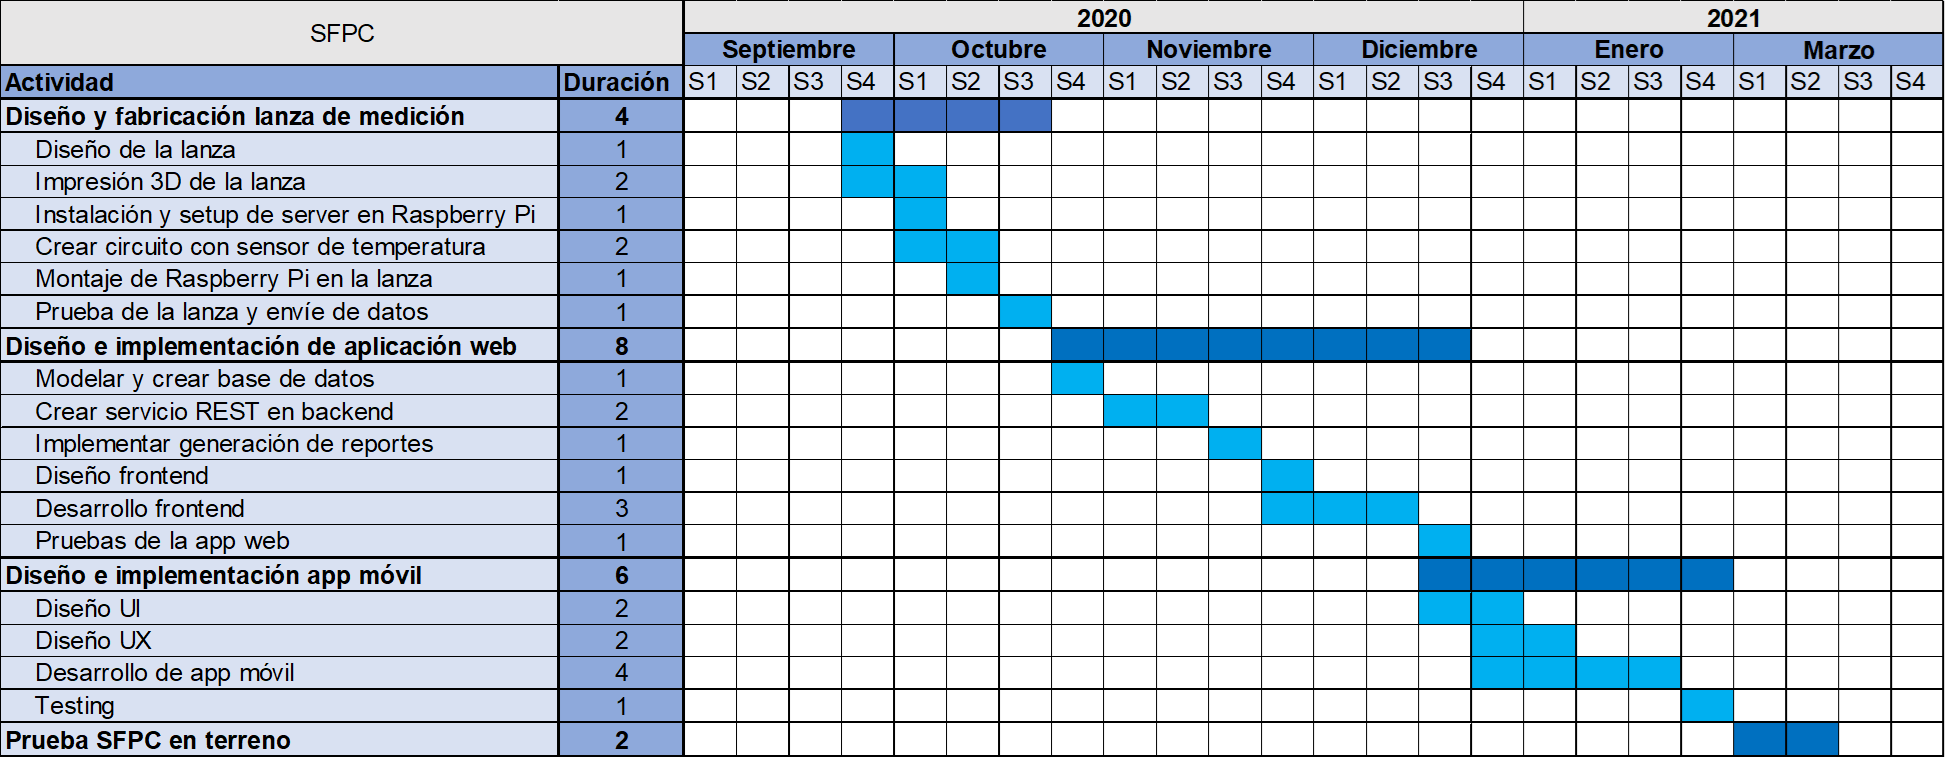
\includegraphics[scale=0.45]{figures/gantt.png}


\section{Bibliografía}
\begin{enumerate}
	\item NCh 2880
	\item "POTENCIALES EFECTOS DE LA AGRICULTURA DIGITAL SOBRE EL MERCADO LABORAL AGROPECUARIO". Oficina de Estudios y Políticas Agrarias, Ministerio de Agricultura
	\item Sistema Nacional de Certificación de Productos Orgánicos Agrícolas. SERVICIO AGRÍCOLA Y GANADERO, DIVISIÓN DE PROTECCIÓN DE LOS RECURSOS NATURALES RENOVABLES. Subdepartamento Agricultura Orgánica
	\item \href{http://www.sag.cl/ambitos-de-accion/sistema-de-auto-certificacion-con-fiscalizacion-directa-del-sag}{Sistema de autocertificación con fiscalización directa del SAG}
\end{enumerate}

\end{document}